% ==========================================================
% modelo-artigo.tex 
% Modelo de Artigo Acadêmico
%
% CRIADO POR: José Nilton Silva Lima
% CURRÍCULO LATTES: https://lattes.cnpq.br/9910161133761662
%
% SOBRE O MODELO:
% Este modelo foi desenvolvido com base na estrutura de artigos
% científicos do Instituto Federal do Piauí (IFPI),
% conforme o manual disponível em:
% https://www.ifpi.edu.br/area-do-estudante/bibliotecas/manual-de-trabalhos-academicos
% (Versão Artigo).
%
% REFERÊNCIAS:
% A estrutura de referências deste modelo segue a norma
% ABNT NBR 6022:2018.
% A versão LaTeX das Referências foi desenvolvida com base no grupo abnTeX2:
% http://www.abntex.net.br/
%
% RECOMENDAÇÃO:
% Para melhor compatibilidade e geração correta do PDF,
% recomenda-se utilizar o compilador **pdfLaTeX** em versão 2024.
%
% COPYRIGHT:
% © 2025 José Nilton Silva Lima. Todos os direitos reservados.
% É permitida a cópia, distribuição e modificação deste código
% para fins acadêmicos, desde que mantidos os créditos originais.
% Uso comercial proibido sem autorização prévia do autor.
% ==========================================================

\documentclass[a4paper,12pt]{article}
\usepackage{artigotemplate}

% === DADOS DO ARTIGO ===
\titulo{TÍTULO DO ARTIGO: Subtítulo do artigo}
\autor{José Nilton Silva Lima}
\instituicao{Instituto Federal de Educação, Ciência e Tecnologia do Piauí}
\campus{Campus Piripiri}
\curso{Tecnólogo em Análise e Desenvolvimento de Sistemas}
\cidade{Piripiri/PI}
\ano{2026}
\orientador{Prof. Dr. Nome do(a) Orientador(a)}
% Caso o trabalho tenha coorientador, retire os comentários das respectivas linhas abaixo.
%\coorientador{Prof. Me. Nome do(a) Coorientador(a)}

% Comente \notaautor e \notaorientador para retirar as notas de rodapé.
\notaautor{Discente do curso de Análise e Desenvolvimento de Sistemas (IFPI); Bolsista da FAPEPI.}
\notaorientador{Docente orientador do IFPI - Campus Piripiri.}
%\notacoorientador{Docente orientador do IFPI - Campus Piripiri.}

% ===========================
% === INÍCIO DO DOCUMENTO ===
% ===========================
\begin{document}

% === CAPA E CONTRACAPA ===
% Os comandos abaixo geram automaticamente a capa e contracapa. Caso queira retirar capa e contracapa, comente os comandos abaixo.
\capaartigo
\clearpage
\contracapaartigo
\clearpage

% === INÍCIO DO CONTEÚDO DO ARTIGO ===
\iniciarpaginacao
\infoartigo

% === RESUMO DO ARTIGO ===
\resumo{
Escreva aqui o resumo do artigo.
}{
palavra-chave 01, palavra-chave 02, palavra-chave 03.
}

% === ABSTRACT DO ARTIGO ===
\abstracten{
Traduza aqui o resumo para o inglês.
}{
Keywords 01, Keywords 02, Keywords 03.
}

% ====================================================
\dataaprovacao{xx/xx/xxxx} % Substitua pela data da aprovação do artigo.

% ====================================================
\section{Introdução}

A introdução apresenta o tema, sua relevância e os objetivos da pesquisa. Contextualize o problema e justifique o estudo. Para
incluir citações no texto, utilize os comandos: De acordo com \citeonline{cassal2021} ou .

% ====================================================
\section{Referencial Teórico}
Apresente o embasamento teórico que sustenta a pesquisa.
Descreva as principais teorias, autores e estudos relacionados ao tema \cite{nussenzveig2013}.

% ====================================================
\subsection{Exemplo de Subseção}
Use subseções para organizar melhor o conteúdo teórico.

% ====================================================
\subsubsection{Exemplo de Subsubseção}
Use subsubseções apenas quando necessário para detalhar tópicos específicos.

Como fazer uma citação direta:
\begin{citacaodireta}
Inclua aqui o trecho exato retirado da fonte, seguido da referência.
Inclua aqui o trecho exato retirado da fonte, seguido da referência.
Inclua aqui o trecho exato retirado da fonte, seguido da referência.
Inclua aqui o trecho exato retirado da fonte, seguido da referência.
Inclua aqui o trecho exato retirado da fonte, seguido da referência \cite[p.~5]{nussenzveig2013}. 
\end{citacaodireta}

% ====================================================
\section{Metodologia}
Descreva detalhadamente como a pesquisa foi conduzida.
Inclua o tipo de pesquisa, materiais utilizados, métodos de coleta e análise de dados, e o procedimento adotado.

% === FIGURA EXEMPLO ===
\begin{figuraCustom}{Exemplo de como inserir uma imagem.}
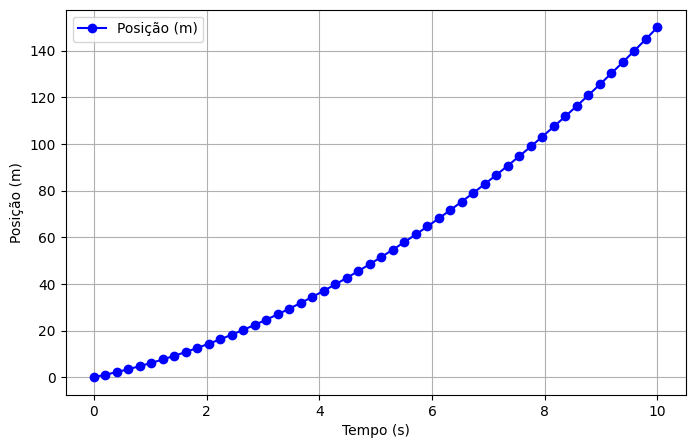
\includegraphics[width=0.5\linewidth]{imagens/imagem_exemplo.png}
\fonte{Elaborado pelos autores.}
\end{figuraCustom}

% === TABELA EXEMPLO ===
\begin{tabelaCustom}{Exemplo de uma tabela.}
\begin{tabular}{c|c|c}
\hline
Categoria & Média & Desvio Padrão \\
\hline
Grupo 1 & 12.47 & 0.83 \\
Grupo 2 & 15.32 & 1.12 \\
Grupo 3 & 14.05 & 0.97 \\
Grupo 4 & 16.28 & 1.35 \\
\hline
\end{tabular}
\fonte{Elaborado pelos autores.}
\end{tabelaCustom}

% === QUADRO EXEMPLO ===
\begin{quadroCustom}{Exemplo de um Quadro.}
\begin{tabular}{|p{5cm}|p{8cm}|}
\hline
\textbf{Coluna 1} & \textbf{Coluna 2} \\
\hline
Descrição detalhada do elemento A, podendo conter múltiplas linhas de texto. &
Conteúdo explicativo associado ao elemento A, com detalhamento técnico ou observações adicionais. \\
\hline
Descrição do elemento B, incluindo informações complementares relevantes. &
Informações adicionais sobre o elemento B, podendo conter dados numéricos, interpretações ou observações críticas. \\
\hline
\end{tabular}
\fonte{Elaborado pelos autores.}
\end{quadroCustom}

% === CÓDIGO EXEMPLO ===
\begin{citacaoCodigo}[Exemplos de Linhas de códigos.]
\begin{blocoDeCodigo}
function main(): void {
  const mensagem: string = "Hello, World!";
  console.log(mensagem);
}

main();
\end{blocoDeCodigo}
\fonte{Elaborado pelos autores.}
\end{citacaoCodigo}

% ====================================================
\section{Resultados e Discussão}
Apresente os resultados obtidos, preferencialmente com apoio de tabelas, gráficos ou figuras.
Interprete e discuta os resultados à luz do referencial teórico.

% ====================================================
\section{Conclusões e Trabalhos Futuros}
Resuma as principais conclusões da pesquisa.
Indique limitações do estudo e sugestões para trabalhos futuros.

% === REFERÊNCIAS ===
\bibliography{referencias} % O arquivo "referencias.bib" deve conter todas as citações utilizadas no texto.

% === APÊNDICES ===
\apendice{A}{Título do Apêndice}
Texto ou conteúdo do apêndice...

% === ANEXOS ===
\anexo{A}{Título do Anexo}
Texto ou conteúdo do anexo...

\anexo{B}{Título do Anexo}
Texto ou conteúdo do anexo...

% ========================
% === FIM DO DOCUMENTO ===
% ========================
\end{document}
